\documentclass[notitlepage,11pt]{article}
\usepackage[margin=1in]{geometry}
\usepackage{enumitem}
\usepackage{textcomp}
\usepackage{amsmath}
\usepackage{graphicx}
\usepackage{listings}
\usepackage{color}
\usepackage{float}

\definecolor{codegreen}{rgb}{0,0.6,0}
\definecolor{codegray}{rgb}{0.5,0.5,0.5}
\definecolor{codepurple}{rgb}{0.58,0,0.82}
\definecolor{backcolour}{rgb}{0.95,0.95,0.92}
 
\lstdefinestyle{mystyle}{
    backgroundcolor=\color{backcolour},   
    commentstyle=\color{codegreen},
    keywordstyle=\color{magenta},
    numberstyle=\tiny\color{codegray},
    stringstyle=\color{codepurple},
    basicstyle=\footnotesize,
    breakatwhitespace=false,         
    breaklines=true,                 
    captionpos=b,                    
    keepspaces=true,                 
    numbers=left,                    
    numbersep=5pt,                  
    showspaces=false,                
    showstringspaces=false,
    showtabs=false,                  
    tabsize=2
}

\lstset{style=mystyle}

\linespread{1.5}
\setlength{\parindent}{1cm} % Default is 15pt.

\title{Capstone Project Report}
\author{Robbie Merillat : RFID Scanning and User Managment}
\author{Robert Schreibman : Game Integration and Housing Construction}
\date{\today}

\begin{document}
    \maketitle
    \begin{abstract}
        In order to speed up the process of logging into an account with a 
        username and password, this project uses an RFID reader which is 
        used to scan a wallet-sized RFID card in order to automatically log 
        into a gaming account. The gaming data and account information is then 
        centrally stored in a file where the associated user can access it either 
        via RFID card tag or using a regular username and password.
    \end{abstract}

    \newpage

    \section{Project Description}
        The broad idea behind this project is to speed up a process of logging into 
        an account. In today’s society, just about every website we visit has required 
        an account set up with a unique username and password. After setting up dozens of 
        these accounts, each with different info, it becomes impossible to remember each 
        specific username and password for every individual website. For convenience, 
        many individuals have allotted this task to third party password managers to 
        keep track of this information. However, for those who do not trust third 
        party password managers, we have created an alternative system that will do 
        the same job. Using an RFID reader, we have interfaced wallet-sized RFID 
        cards with account login information. 

        Currently, our system is interfaced with a single account associated with two terminal games. After a user scans their RFID card, they will be automatically logged into their account where their game statistics are kept per game. The user then can choose one of two games: tic tac toe or four in a row. After playing their game statistics will be saved to their RFID account.
    \section{Sensors}

        The primary sensor used in this project is an RFID reader chip. This 
        chip can scan RFID tags from two inches away through a 3D printed death 
        star case made out of polylactic acid (PLA) material. Each RFID card comes 
        with a unique serial tag that the RFID reader will scan and save to a file. 
        The RFID reader is safely stored inside the death star case as shown in Figure 
        \ref{fig:death}.

        \begin{figure}[h]
            \centering
            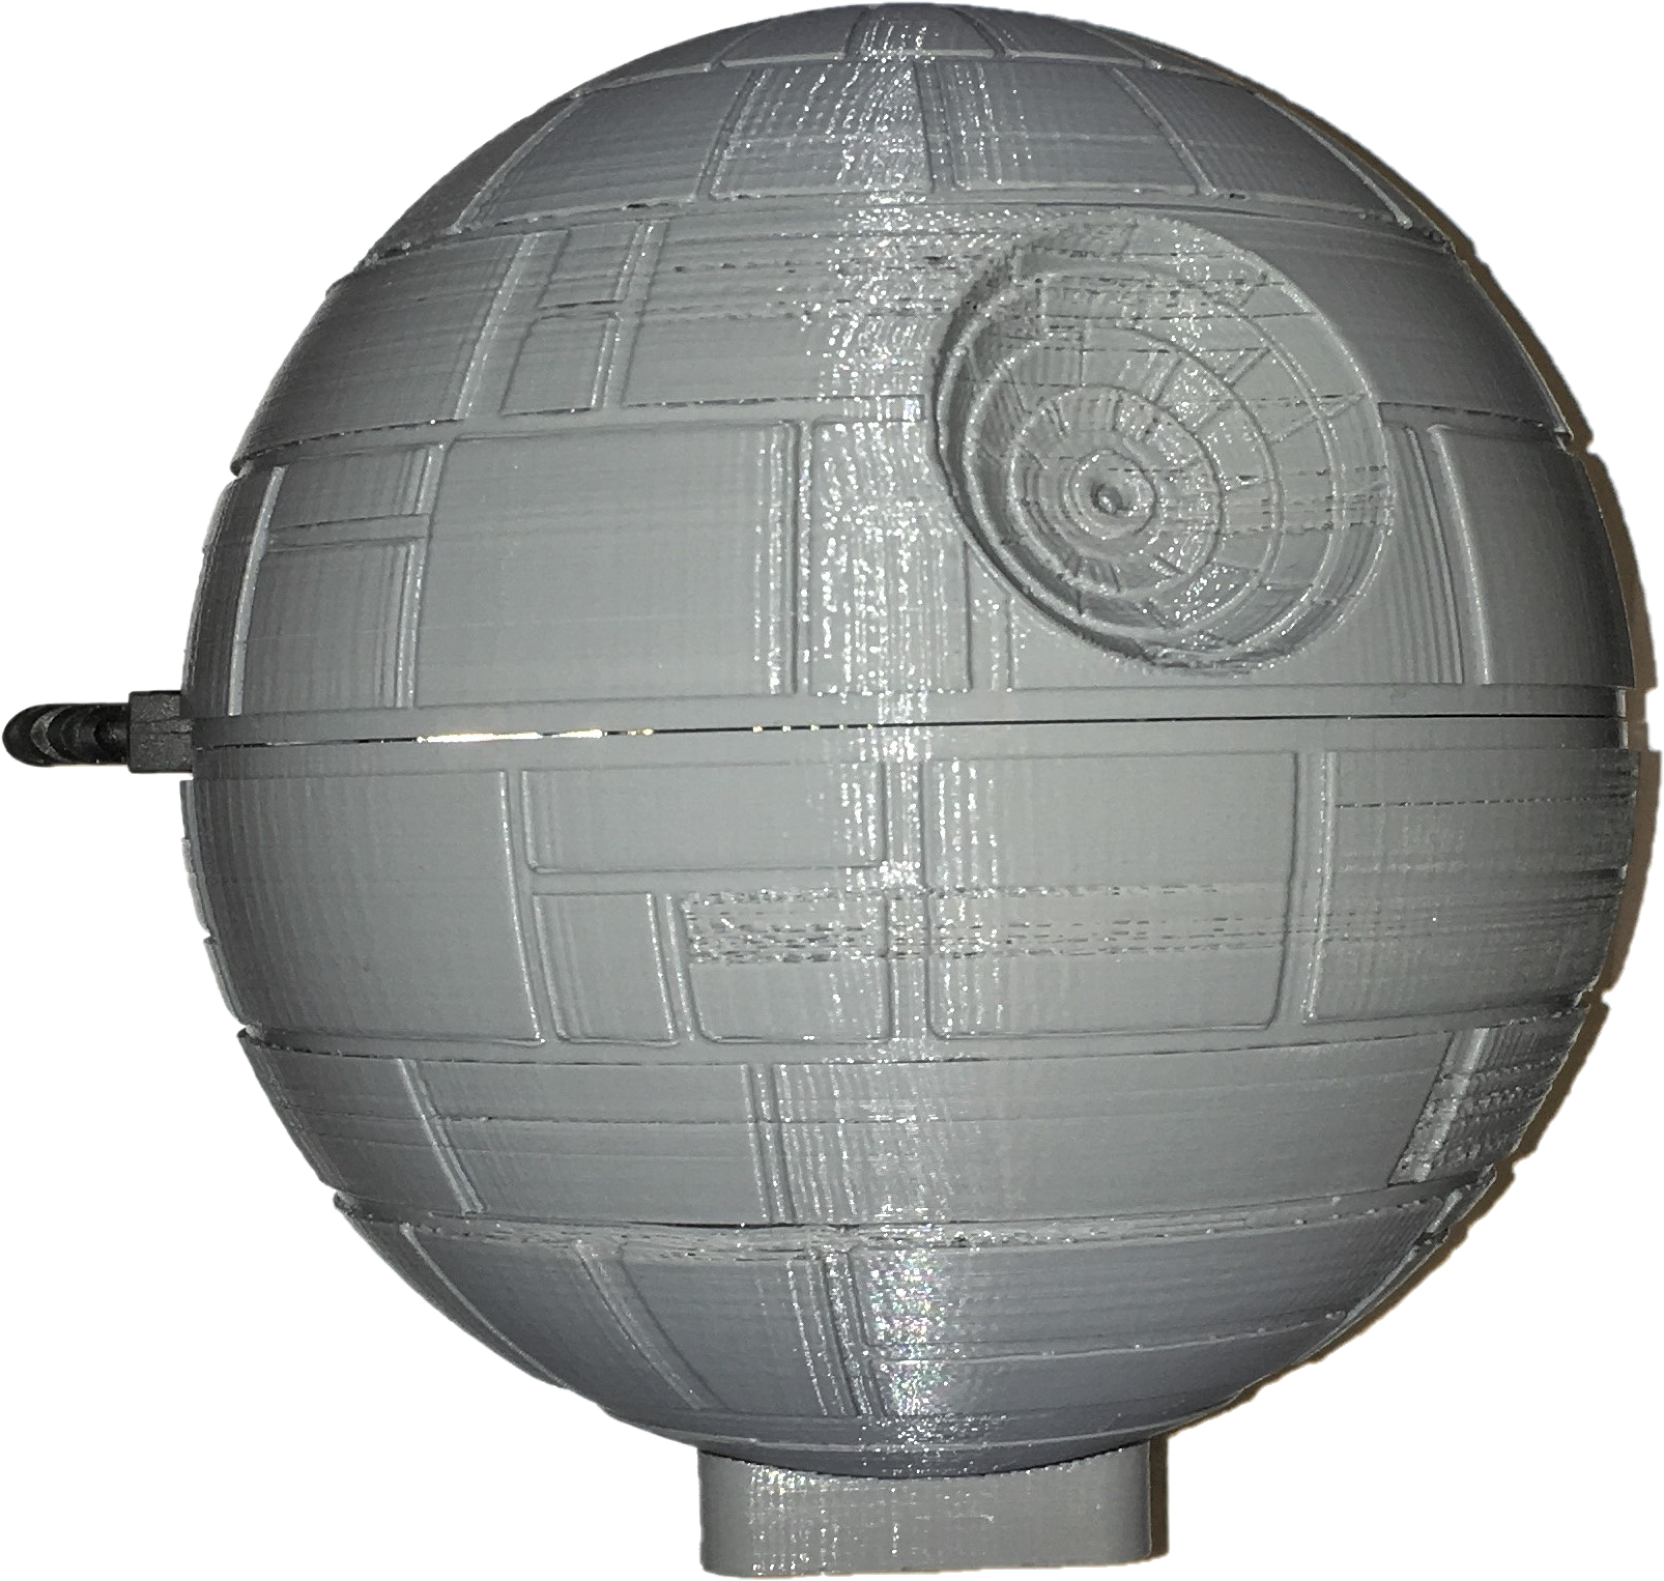
\includegraphics[width=0.5\textwidth]{images/deathstar.png}
            \caption{Raspberry Pi Death Star case 3D printed using PLA}
            \label{fig:death}
        \end{figure}

        
    \section{Obstacles}

        The proposed scope of the project included four main parts. The first 
        part was to get the RFID reader to first successfully recognize tags. 
        After receiving the RFID starter kit, we had trouble trying to figure out 
        how to read from the pins on the RFID reader. We never figured it out, so 
        instead, we decided to interface the RFID reader with the raspberry pi over 
        a USB connection since there was more documentation on doing this, and this is 
        a much more user-friendly connection setup. The circuit diagram for this wired 
        connection is shown in Figure X. The next part was to get the Raspberry Pi 
        to maintain a history of previously scanned RFID cards so new users could 
        create login profiles. This was done by writing to a file a list of scanned 
        RFID tags. If a recognized tag was scanned, then the Raspberry Pi would 
        just load the user data from the file. The third part of this project was 
        to interface the user data with multiple games. We were able to integrate 
        Tic Tac Toe and Four In a Row into a menu list of games to play. The 
        terminal interface of these two games is shown in Figures \ref{fig:ticCommand} 
        and \ref{fig:fourCommand}. The fourth part of our project was to save the 
        game data into a central location which is saved under the current user 
        logged on.

        After the game exits successfully, it returns the results of the game 
        which is then updated to the current users' statistics

        \begin{figure}[h]
            \centering
            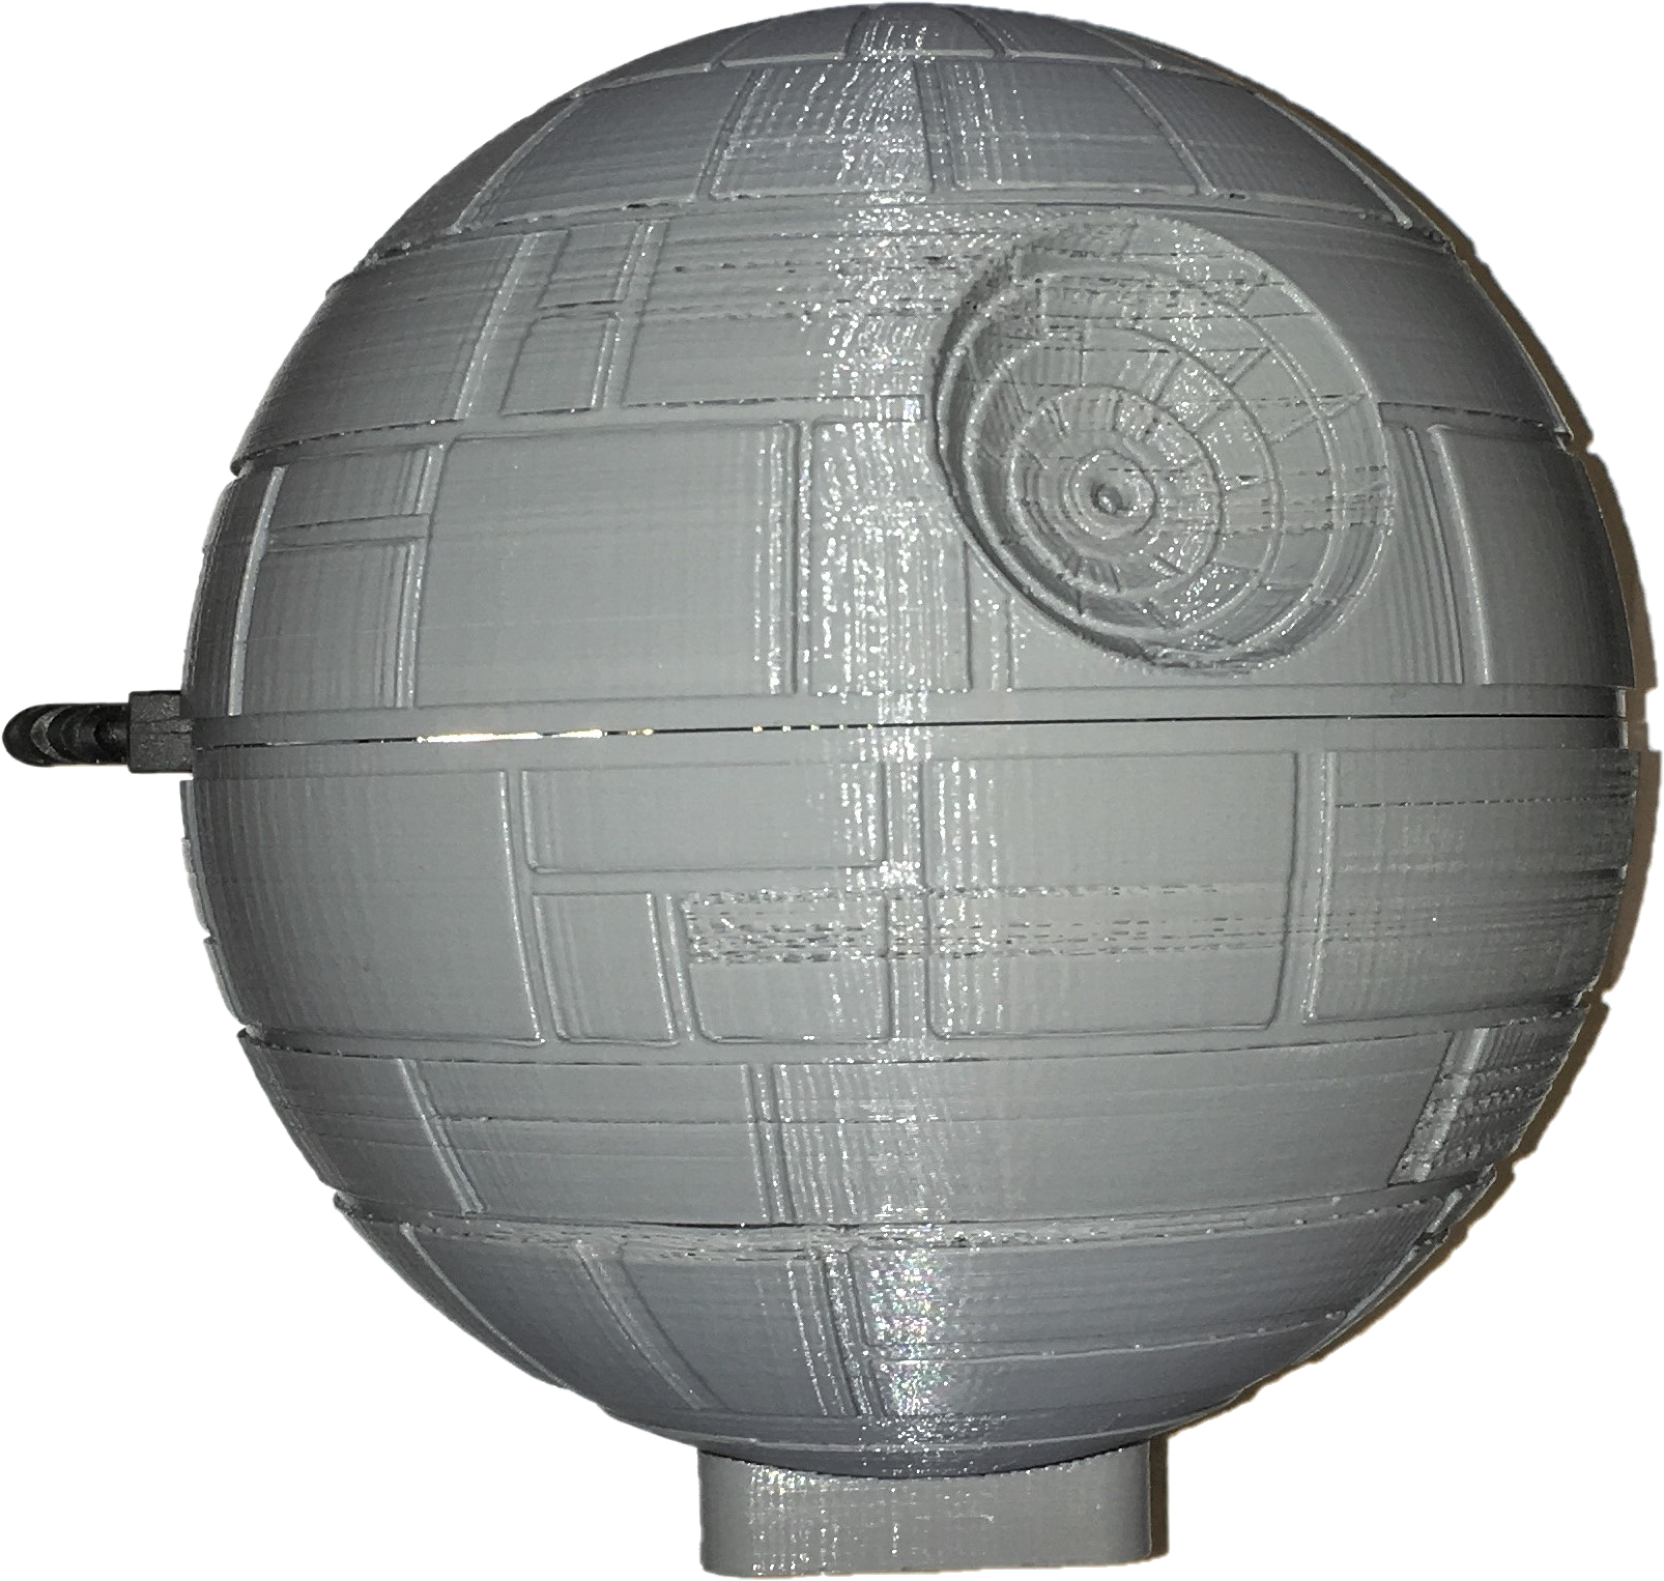
\includegraphics[width=0.5\textwidth]{images/deathstar.png}
            \caption{Tic Tac Toe Command Line Interface}
            \label{fig:ticCommand}
        \end{figure}

        \begin{figure}[h]
            \centering
            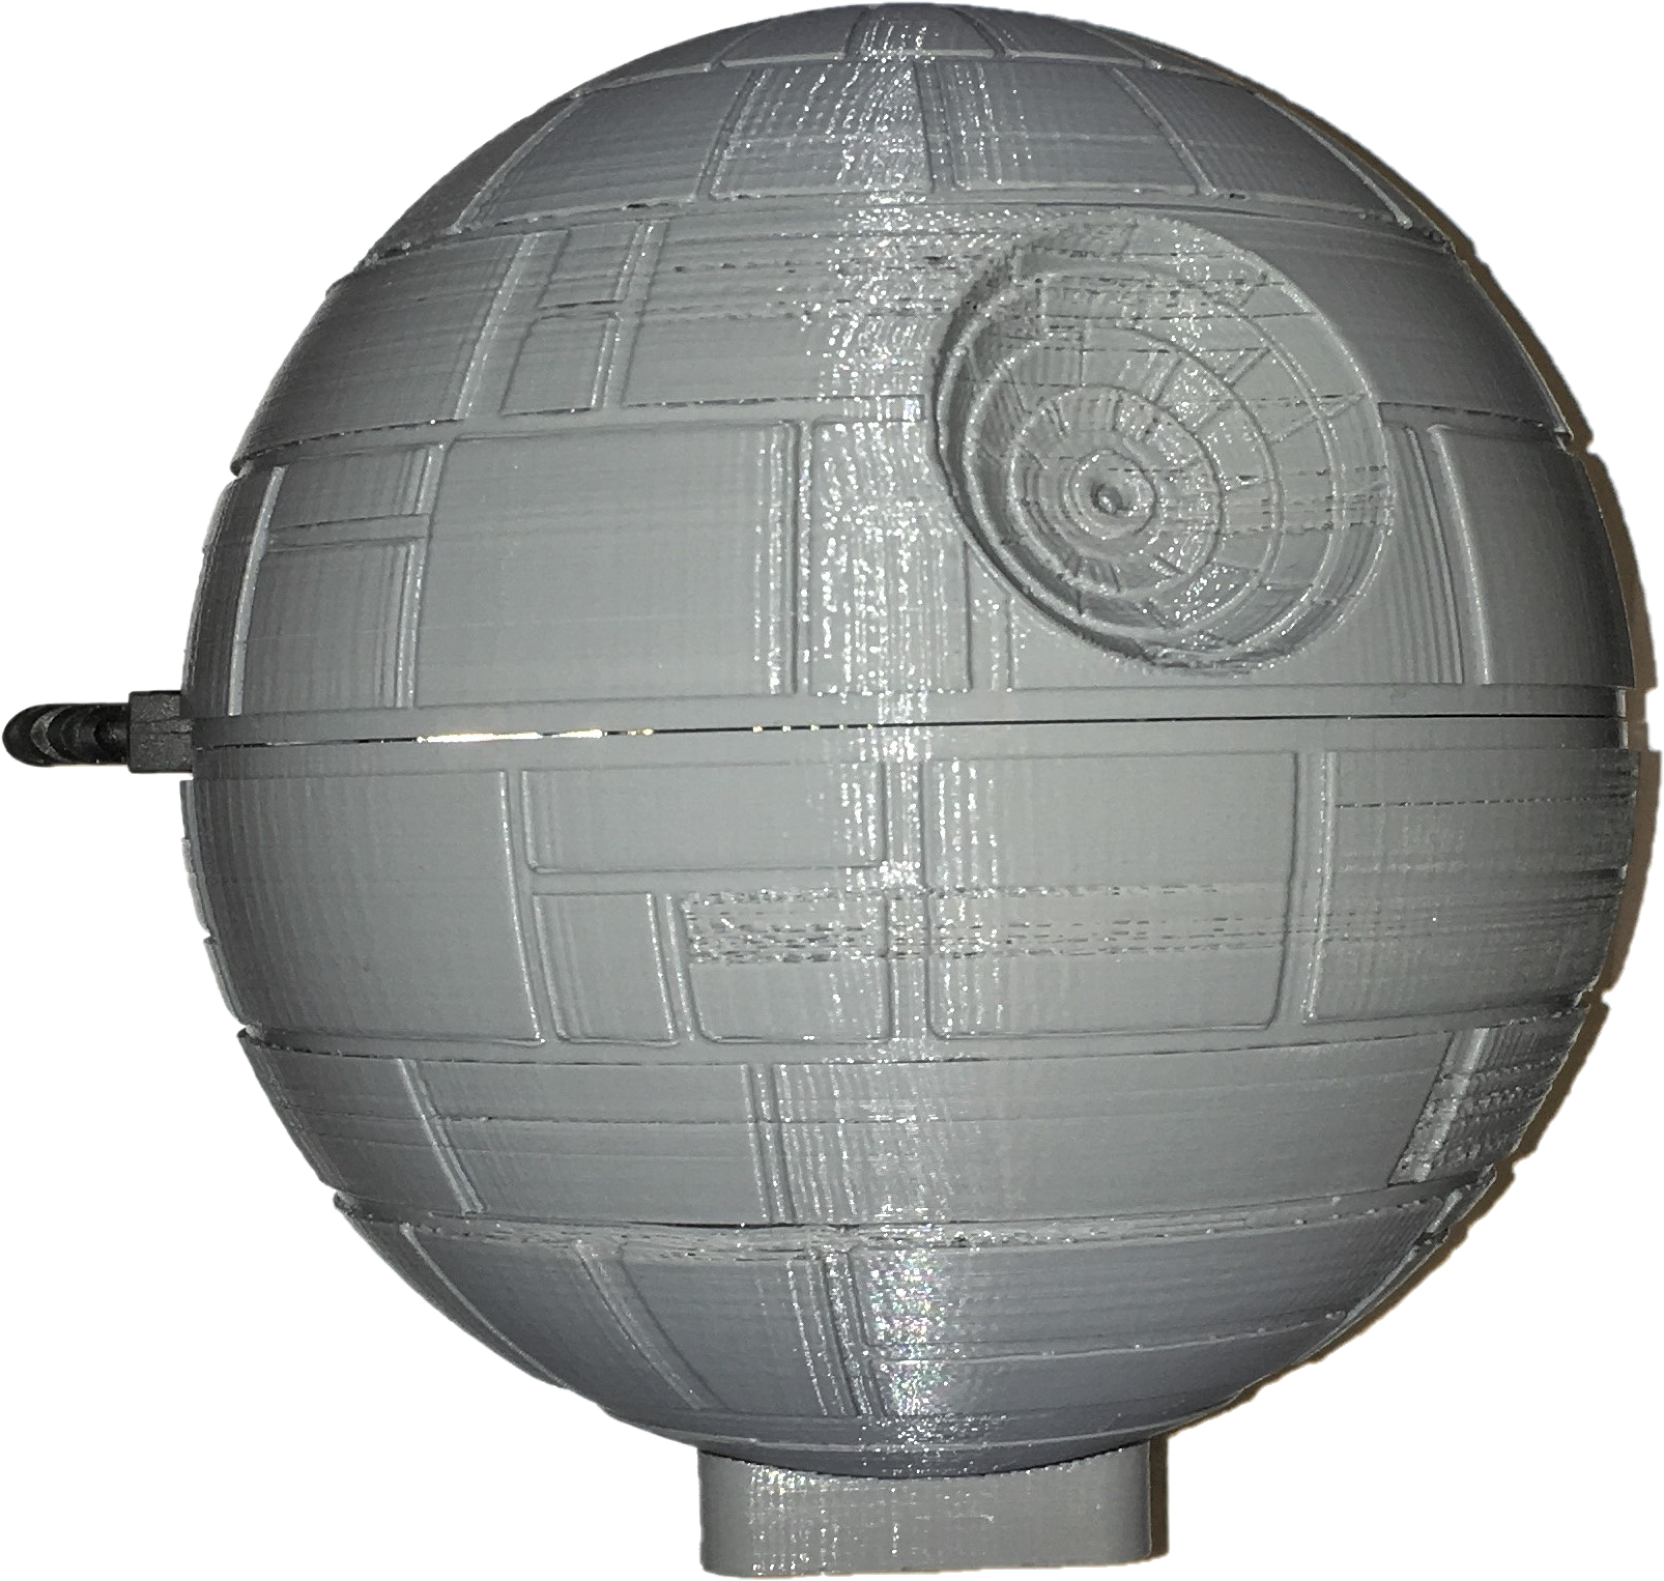
\includegraphics[width=0.5\textwidth]{images/deathstar.png}
            \caption{ Four In a Row Command Line Interface}
            \label{fig:fourCommand}
        \end{figure}

    \section{Results}

    \section{Summary}

    \section{Code}
        \textbf{"run.py begins our code and starts the RFID reader"}
        \lstinputlisting[language=Python]{../run.py}

\end{document}
